\pdfminorversion=4
\documentclass[aspectratio=169]{beamer}

\mode<presentation>
{
  \usetheme{default}
  \usecolortheme{default}
  \usefonttheme{default}
  \setbeamertemplate{navigation symbols}{}
  \setbeamertemplate{caption}[numbered]
  \setbeamertemplate{footline}[frame number]  % or "page number"
  \setbeamercolor{frametitle}{fg=white}
  \setbeamercolor{footline}{fg=black}
} 

\usepackage[english]{babel}
\usepackage[utf8x]{inputenc}
\usepackage{tikz}
\usepackage{courier}
\usepackage{array}
\usepackage{bold-extra}
\usepackage{minted}
\usepackage[thicklines]{cancel}
\usepackage{fancyvrb}

\xdefinecolor{dianablue}{rgb}{0.18,0.24,0.31}
\xdefinecolor{darkblue}{rgb}{0.1,0.1,0.7}
\xdefinecolor{darkgreen}{rgb}{0,0.5,0}
\xdefinecolor{darkgrey}{rgb}{0.35,0.35,0.35}
\xdefinecolor{darkorange}{rgb}{0.8,0.5,0}
\xdefinecolor{darkred}{rgb}{0.7,0,0}
\definecolor{darkgreen}{rgb}{0,0.6,0}
\definecolor{mauve}{rgb}{0.58,0,0.82}

\title[2019-06-18-cmsml3-uproot]{Uproot: accessing ROOT data in the scientific Python ecosystem}
\author{Jim Pivarski}
\institute{Princeton University -- IRIS-HEP}
\date{June 18, 2019}

\usetikzlibrary{shapes.callouts}

\begin{document}

\logo{\pgfputat{\pgfxy(0.11, 7.4)}{\pgfbox[right,base]{\tikz{\filldraw[fill=dianablue, draw=none] (0 cm, 0 cm) rectangle (50 cm, 1 cm);}\mbox{\hspace{-8 cm}
\includegraphics[height=1 cm]{princeton-logo-long.png}\hspace{0.1 cm}\raisebox{0.1 cm}{
\includegraphics[height=0.8 cm]{iris-hep-logo-long.png}}\hspace{0.1 cm}}}}}

\begin{frame}
  \titlepage
\end{frame}

\logo{\pgfputat{\pgfxy(0.11, 7.4)}{\pgfbox[right,base]{\tikz{\filldraw[fill=dianablue, draw=none] (0 cm, 0 cm) rectangle (50 cm, 1 cm);}\mbox{\hspace{-8 cm}
\includegraphics[height=1 cm]{princeton-logo.png}\hspace{0.1 cm}\raisebox{0.1 cm}{
\includegraphics[height=0.8 cm]{iris-hep-logo.png}}\hspace{0.1 cm}}}}}

% Uncomment these lines for an automatically generated outline.
%\begin{frame}{Outline}
%  \tableofcontents
%\end{frame}

% START START START START START START START START START START START START START

\begin{frame}{Python is the primary interface for machine learning these days}
\vspace{0.5 cm}

\mbox{ } 
\includegraphics[height=0.8 cm]{sklearn-logo.png}
\hfill 
\includegraphics[height=0.8 cm]{pytorch-logo.png}
\hfill 
\includegraphics[height=0.8 cm]{keras-logo.png}
\hfill 
\includegraphics[height=1 cm]{tensorflow-logo.png}
\hfill 
\includegraphics[height=0.8 cm]{caffe2-logo.png}
\hfill 
\includegraphics[height=0.8 cm]{gluon-logo.png} \mbox{ }

\mbox{ } 
\includegraphics[height=0.8 cm]{chainer-logo.png}
\hfill 
\includegraphics[height=1 cm]{cntk-logo.png}
\hfill 
\includegraphics[height=0.8 cm]{lasagne-logo.png}
\hfill 
\includegraphics[height=0.6 cm]{onnx-logo.png}
\hfill 
\includegraphics[height=0.8 cm]{cesium-logo.png}
\hfill 
\includegraphics[height=0.8 cm]{xgboost-logo.png} \mbox{ }

\vspace{1 cm}
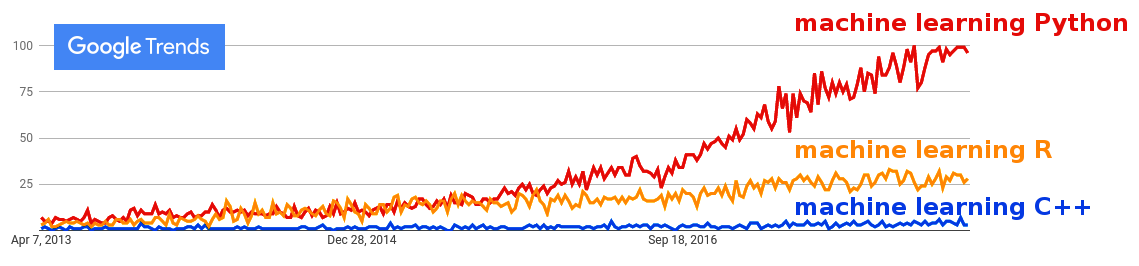
\includegraphics[width=\linewidth]{python-r-cpp-googletrends-machinelearning.png}
\end{frame}

\begin{frame}{ROOT data in Python: three approaches}
\vspace{0.3 cm}
\large
\begin{enumerate}
\item \textcolor{darkblue}{PyROOT:} new methods for direct TTree-to-Numpy translation.
\item \textcolor{darkblue}{root\_numpy:} Python/C++ extension module, compiles into ROOT.
\item \textcolor{darkblue}{uproot:} independent ROOT I/O implementation in Python.
\end{enumerate}

\vspace{0.2 cm}
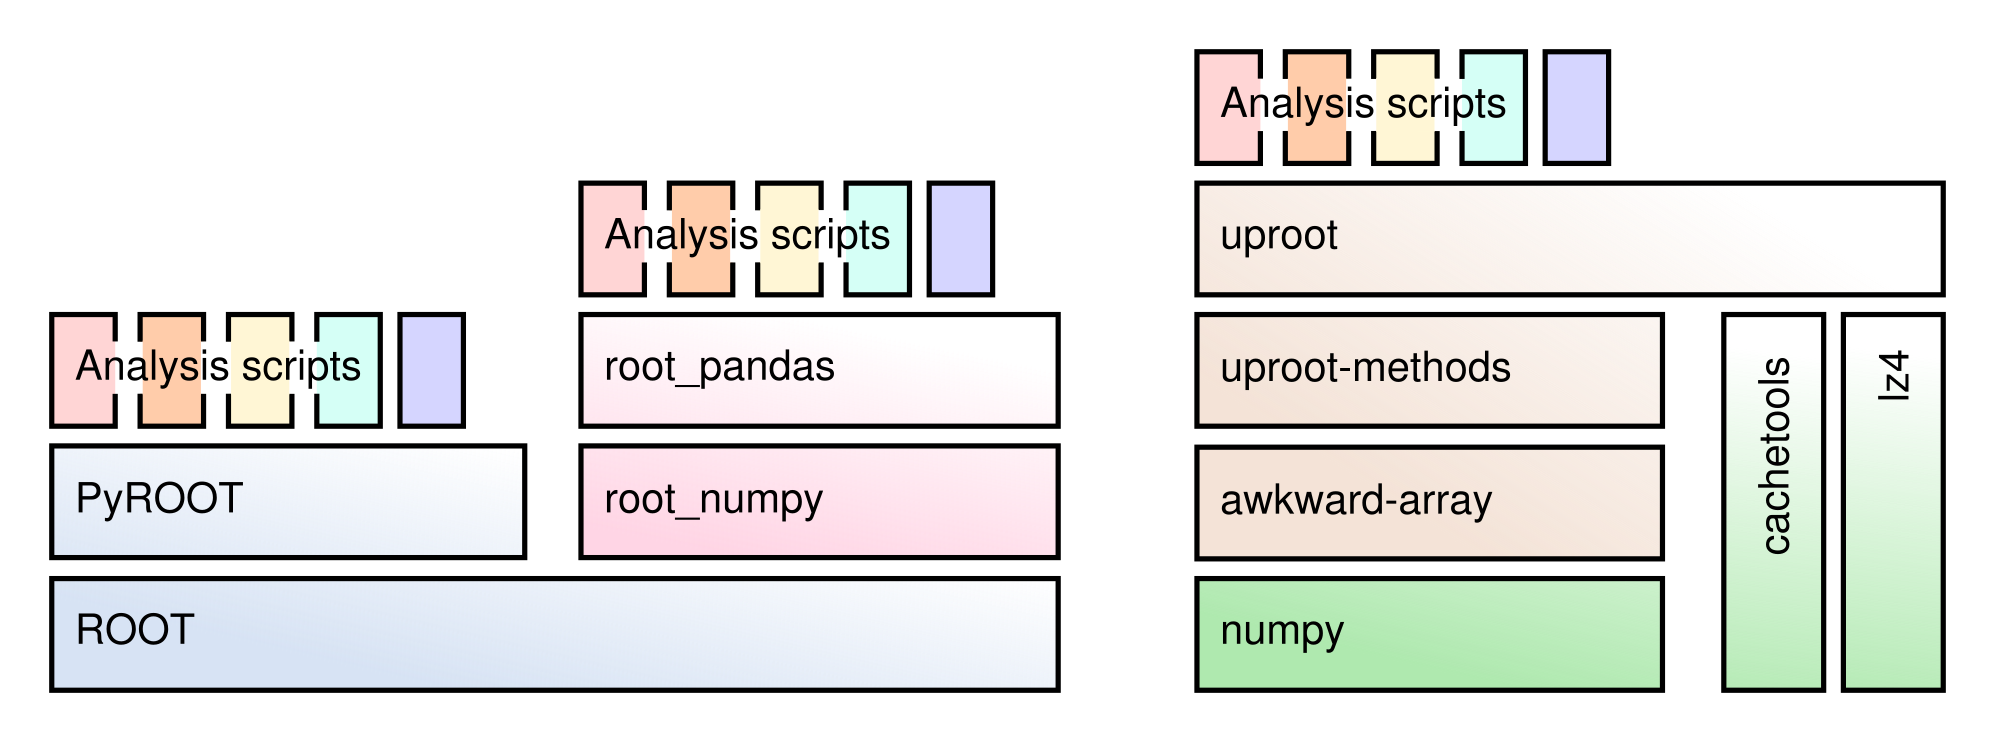
\includegraphics[width=\linewidth]{abstraction-layers.png}
\end{frame}

\begin{frame}{}
\LARGE
\begin{center}
Approach \#1: \textcolor{darkblue}{PyROOT}
\end{center}
\end{frame}

\begin{frame}[fragile]{PyROOT's universal bindings are great, but slow$^2$}
\vspace{0.5 cm}
PyROOT is unique among Python-C++ bindings in that no manual association of Python objects to C++ objects is required (thanks to ROOT/Cling's C++ reflection).

\vspace{0.25 cm}
\small
\begin{minted}{python}
file = ROOT.TFile("cms-nanoaod.root")
tree = file.Get("Events")
tree.SetBranchStatus("*", 0)
tree.SetBranchStatus("nMuon", 1)
tree.SetBranchStatus("Muon_pt", 1)
tree.SetBranchStatus("Muon_eta", 1)

for event in tree:
    for pt, eta in zip(event.Muon_pt, event.Muon.eta):
        pt * math.sinh(eta)
\end{minted}
\large

\vspace{0.25 cm}
BUT the above is \textcolor{darkblue}{$36\times$ slower than pure Python} (and $1000\times$ slower than C++) because of reflection {\it in the loop.}
\end{frame}

\begin{frame}[fragile]{New methods to go directly to Numpy}
\large
\vspace{0.5 cm}
New ``Pythonizations'' are being added to PyROOT for useful features like {\tt AsMatrix}, which fill an array on the C++ side, without reflection.

\small
\begin{minted}{python}
tree.AsMatrix(["MET_px", "MET_py"])
\end{minted}
\begin{verbatim}
array([[  5.91277122,   2.5636332 ],
       [ 24.76520348, -16.34910965],
       [-25.78508759,  16.23713112],
       ...,
       [ 18.10164642,  50.29071808],
       [ 79.87519073, -52.35145187],
       [ 19.71374893,  -3.59541821]])
\end{verbatim}
\large

\vspace{0.25 cm}
The return type is an unlabeled matrix, but you can ask for the labels explicitly (e.g.\ to make a Pandas DataFrame).

\small
\begin{minted}{python}
data, labels = tree.AsMatrix(["MET_px", "MET_py"], return_labels=True)
pandas.DataFrame(data, columns=labels)
\end{minted}
\end{frame}

\begin{frame}[fragile]{However, {\tt AsMatrix} is only for numeric branches: no collections}
\vspace{0.5 cm}

\small
\begin{minted}{python}
tree.AsMatrix(["Muon_pt"])    # arbitrary number of muons per event
\end{minted}
\begin{verbatim}
array([[0.],
       [0.],
       [0.],
       ...,
       [0.],
       [0.],
       [0.]])
\end{verbatim}

\vspace{-0.2 cm}
\color{gray}
\begin{verbatim}
Error in <TTreeReaderValueBase::GetBranchDataType()>: Must use
TTreeReaderArray to read branch Muon_pt: it contains an array
or a collection.
\end{verbatim}
\begin{verbatim}
Error in <TTreeReaderValueBase::CreateProxy()>: The branch Muon_pt
contains data of type {UNDETERMINED TYPE}, which does not have a
dictionary.
\end{verbatim}
\end{frame}

\begin{frame}{}
\vspace{-0.1 cm}
\begin{columns}
\column{1.145\linewidth}
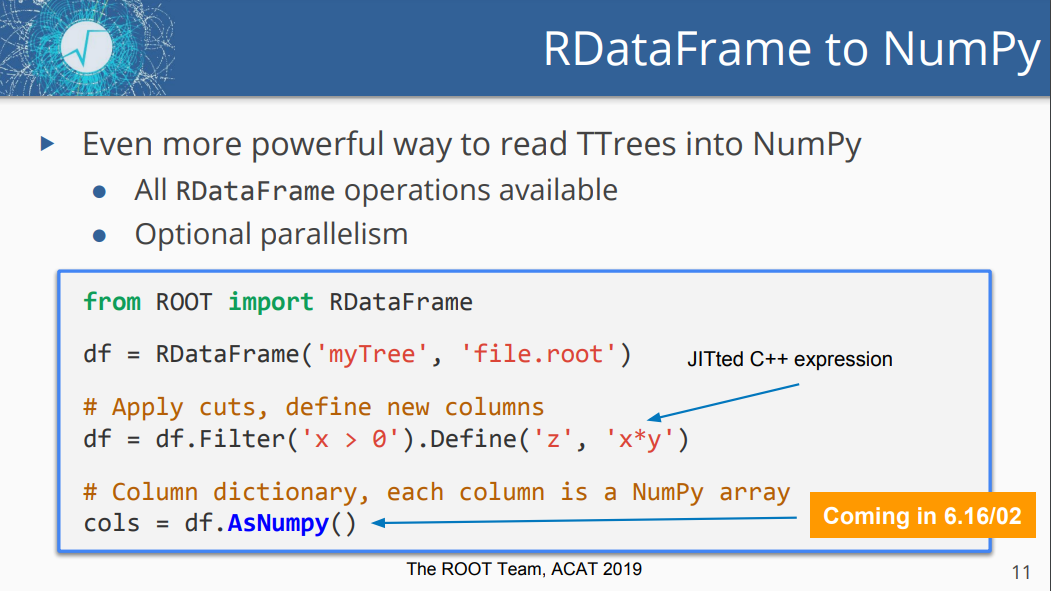
\includegraphics[width=\linewidth]{03-coming-soon-2.png}
\end{columns}
\end{frame}

\begin{frame}{}
\LARGE
\begin{center}
Approach \#2: \textcolor{darkblue}{root\_numpy}
\end{center}
\end{frame}

\begin{frame}[fragile]{root\_numpy compiles into Python and ROOT}
\vspace{0.25 cm}
\small
\begin{minted}{python}
root_numpy.tree2array(tree, ["MET_px", "MET_py"])     # PyROOT "tree"

root_numpy.root2array("cms-nanoaod.root", "Events",   # no PyROOT
                      ["MET_px/1000.0", "MET_py/1000.0"])
\end{minted}
\large

\vspace{0.25 cm}
Any {\tt TTree::Draw} expression may be used, not just branch names, and it's as fast as {\tt TTree::Draw}. You can think of it as ``{\tt TTree::Draw} to Numpy.''

\vspace{0.25 cm}
\mbox{ } \hfill 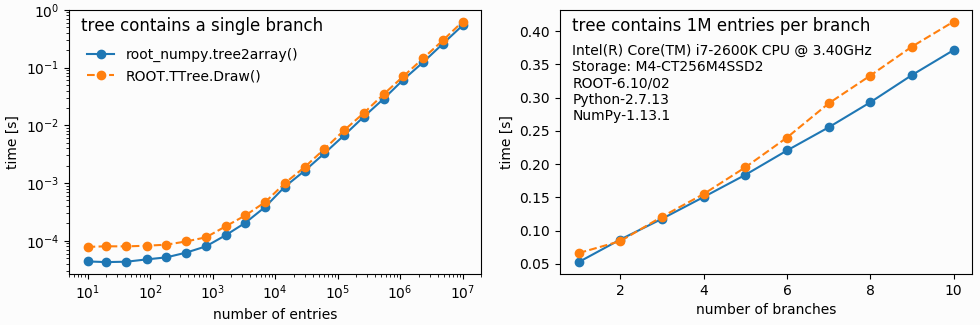
\includegraphics[width=0.8\linewidth]{root-numpy-fast.png} \hfill \mbox{ }
\end{frame}

\begin{frame}[fragile]{Collections in root\_numpy}
\large
\vspace{0.5 cm}

root\_numpy {\it can} read collections of numeric types (``jagged arrays''), but uses the nearest Numpy type: an array whose contents are arrays (i.e. Python objects).

\small
\begin{minted}{python}
root_numpy.tree2array(tree, "Muon_pt")
\end{minted}
\begin{verbatim}
array([array([], dtype=float32),
       array([], dtype=float32),
       array([5.315762], dtype=float32),
       ...,
       array([26.351288], dtype=float32),
       array([], dtype=float32),
       array([44.28051, 6.6997213], dtype=float32)],
      dtype=object)
\end{verbatim}

\large
Undermines the two advantages of Numpy: speed and flexibility (inner arrays are not recognized as a dimension).
\end{frame}

\begin{frame}{}
\begin{columns}
\column{1.145\linewidth}
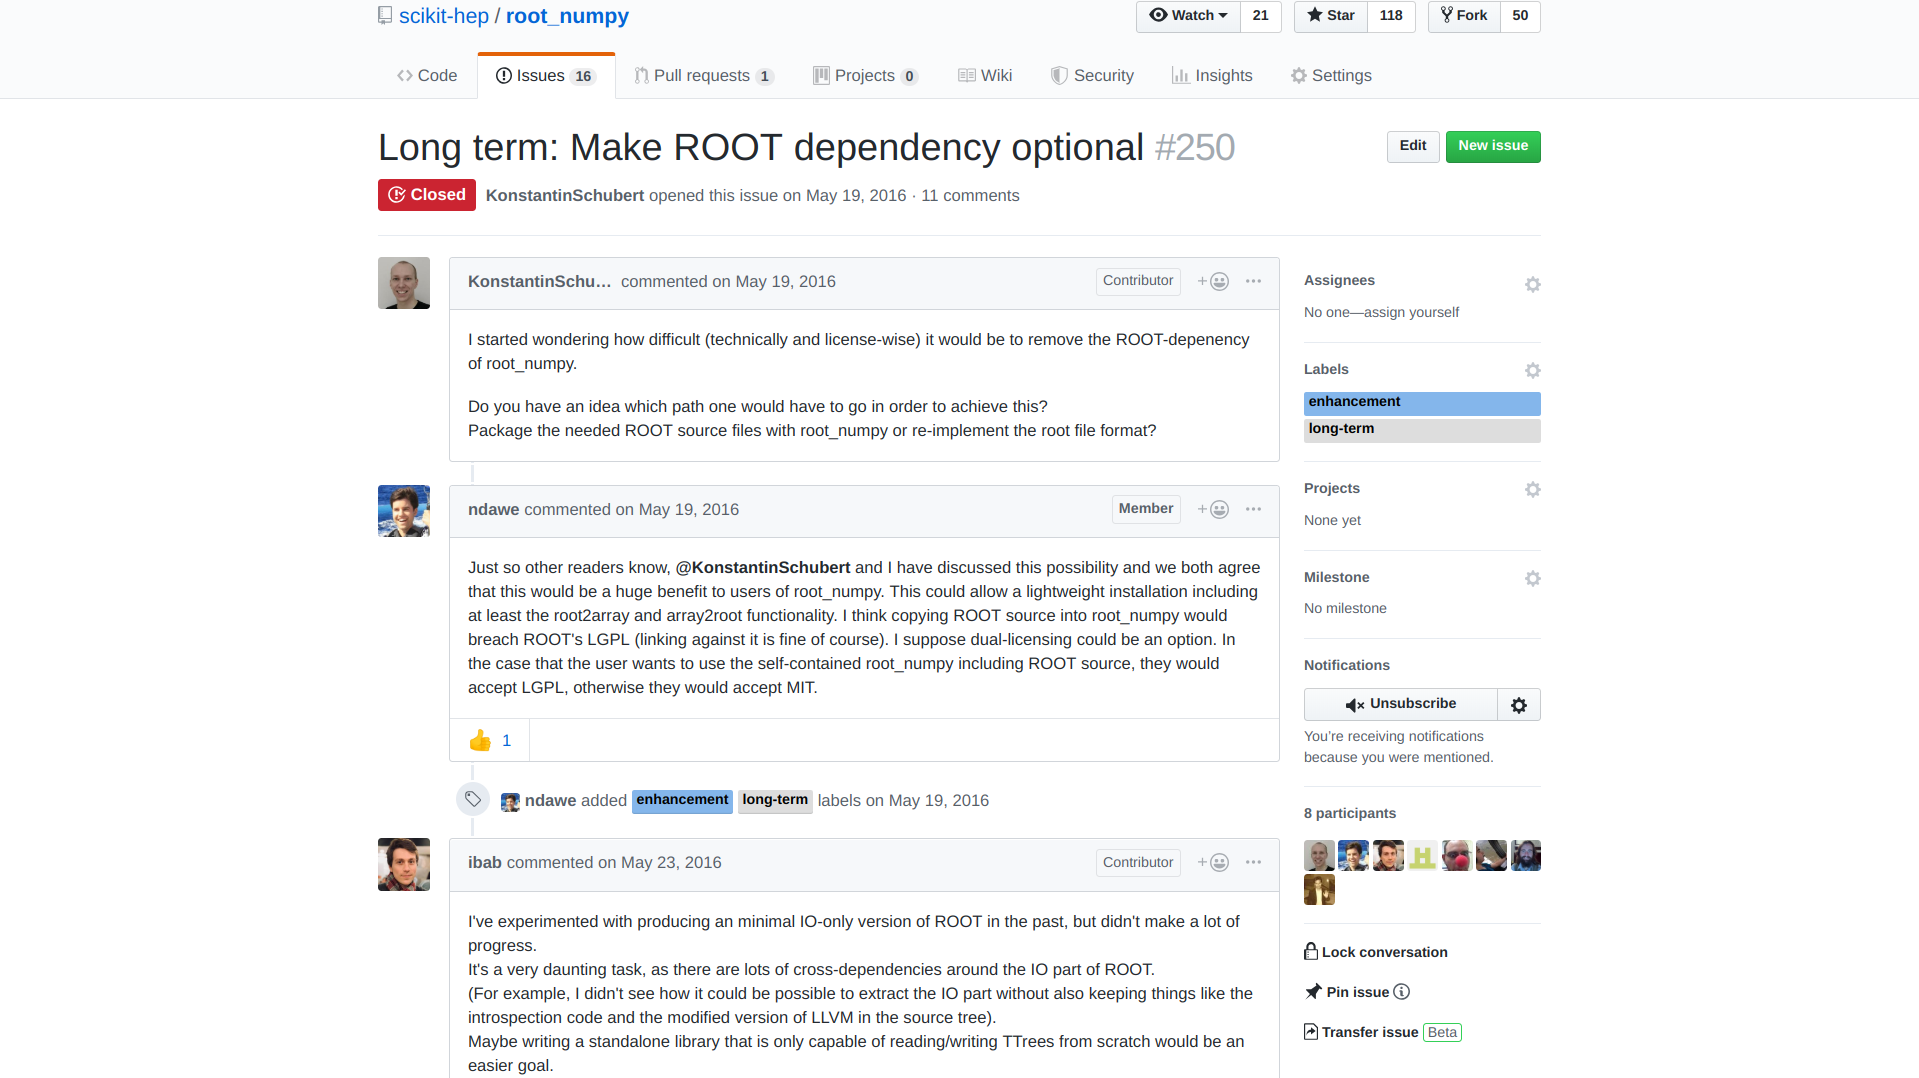
\includegraphics[width=\linewidth]{root-numpy-optionalroot.png}
\end{columns}
\end{frame}

\begin{frame}{}
\LARGE
\begin{center}
Approach \#3: \textcolor{darkblue}{uproot}
\end{center}
\end{frame}

\begin{frame}{}



\end{frame}

\end{document}
